\documentclass[11pt,a4paper]{article}
\usepackage{fontspec}
\setmainfont{DejaVu Sans}[Scale=0.92]
\usepackage{amsmath,amssymb}
\usepackage[left=18mm,right=60mm,top=13mm,bottom=10mm]{geometry}
\usepackage{array,xcolor}
\usepackage{pgfplots}\pgfplotsset{compat=1.16}
\definecolor{grau}{gray}{0.42}
\pagestyle{empty}
\setlength{\parindent}{0pt}
\renewcommand{\arraystretch}{1.38}
\newcommand{\w}[1]{\leavevmode{\small\color{grau}$|$ #1}}
\begin{document}
{\large\bfseries Schema Kurvendiskussion}\hfill{\small\color{grau}Entwurf 3 · 17.10.2026}\par
\vspace{2pt}\hrule height 1.2pt\vspace{6pt}
{\small\color{grau}Stellen: $x_N$ Nullstelle, $x_E$ Extremstelle, $x_W$ Wendestelle, $x_S$ Sattelstelle
(wenn die Aufgabe nichts vorgibt). Punkte: $H(x_E\,|\,f(x_E))$, $T$, $W$, $S$ entsprechend.}
\vspace{6pt}

\begin{tabular}{@{}>{\bfseries}p{2.9cm}p{9.3cm}@{}}
Symmetrie & $f(-x)=f(x)\ \Rightarrow$ achsensymmetrisch zur $y$-Achse\\
 & $f(-x)=-f(x)\ \Rightarrow$ punktsymmetrisch zu $O$\\
 & \w{ganzrational: nur gerade oder nur ungerade Exponenten; Zahl $=a\cdot x^0$ (gerade), $x=x^1$ (ungerade)}\\
Unendlich & $\lim\limits_{x\to\pm\infty} f(x)$ \ \w{ganzrational: führender Term; $\mathrm e^x\to0$ für $x\to-\infty$, $\mathrm e^x\to\infty$ für $x\to+\infty$}\\
Nullstellen & $f(x_N)=0$ \ \w{ausklammern, Nullprodukt, pq- oder abc-Formel; Nullstelle raten, dann Polynomdivision}\\
$y$-Achse & $f(0)$\\
Extrempunkte & zz: $f'(x_E)=0$ (notwendig)\\
 & \quad und $f''(x_E)<0\ \Rightarrow$ H; \ $f''(x_E)>0\ \Rightarrow$ T (hinreichend)\\
 & alt.\ (immer bei $f''(x_E)=0$): VZW von $f'$ bei $x_E$\\
 & \w{VZW: Testwert links und rechts von $x_E$ in $f'$ einsetzen (zwischen den benachbarten Nullstellen von $f'$)}\\
 & \w{kurz, wenn $f'$ in Faktoren steht: $(x-x_E)$ einfach $\Rightarrow$ VZW; $(x-x_E)^2$ doppelt $\Rightarrow$ kein VZW $\Rightarrow$ S}\\
 & \quad $-\to+\ \Rightarrow$ T; \ $+\to-\ \Rightarrow$ H; \ kein VZW $\Rightarrow$ Sattelpunkt\\
 & Punkt: $H(x_E\,|\,f(x_E))$\\
Wendepunkte & zz: $f''(x_W)=0$ (notwendig) und $f'''(x_W)\neq0$ (hinreichend)\\
 & alt.: VZW von $f''$ bei $x_W$\\
 & Punkt: $W(x_W\,|\,f(x_W))$; \ zusätzlich $f'(x_W)=0\ \Rightarrow$ Sattelpunkt\\
Monotonie & $f'>0$ steigt, $f'<0$ fällt; Bereiche zwischen den Extremstellen\\
 & \w{Schreibweise: $f$ steigt auf $]-\infty;x_{E1}]$, fällt auf $[x_{E1};x_{E2}]$ …}\\
Krümmung & $f''>0$ linksgekrümmt, $f''<0$ rechtsgekrümmt; Bereiche zwischen den Wendestellen\\
Tangente & $t(x)=mx+n$; \ $m=f'(x_0)$, \ $n$ aus $t(x_0)=f(x_0)$\\
Wertemenge & aus Grenzwerten und Extrempunkten\\
\end{tabular}

\vspace{8pt}
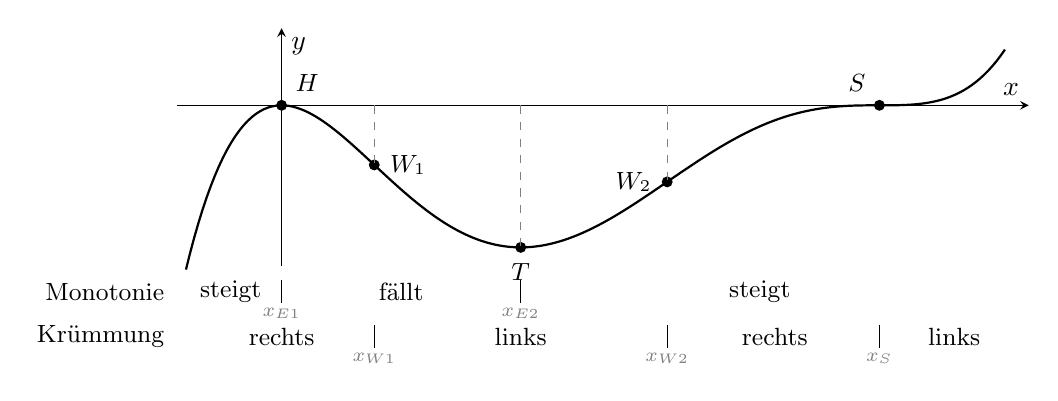
\begin{tikzpicture}
\begin{axis}[width=12.4cm,height=4.6cm,axis lines=middle,xmin=-0.35,xmax=2.5,ymin=-1.25,ymax=0.6,xtick=\empty,ytick=\empty,xlabel={$x$},ylabel={$y$},clip=false]
\addplot[domain=-0.32:2.42,samples=200,thick] {x^2*(x-2)^3};
\node[circle,fill,inner sep=1.4pt,label={[font=\small]north east:$H$}] at (axis cs:0,0) {};
\node[circle,fill,inner sep=1.4pt,label={[font=\small]south:$T$}] at (axis cs:0.8,-1.106) {};
\node[circle,fill,inner sep=1.4pt,label={[font=\small]east:$W_1$}] at (axis cs:0.31,-0.464) {};
\node[circle,fill,inner sep=1.4pt,label={[font=\small]west:$W_2$}] at (axis cs:1.29,-0.596) {};
\node[circle,fill,inner sep=1.4pt,label={[font=\small]north west:$S$}] at (axis cs:2,0) {};
\draw[gray,dashed] (axis cs:0.8,0) -- (axis cs:0.8,-1.106);
\draw[gray,dashed] (axis cs:0.31,0) -- (axis cs:0.31,-0.464);
\draw[gray,dashed] (axis cs:1.29,0) -- (axis cs:1.29,-0.596);
\node[font=\small,anchor=east] at (axis cs:-0.36,-1.45) {Monotonie};
\node[font=\small] at (axis cs:-0.17,-1.45) {steigt};
\node[font=\small] at (axis cs:0.4,-1.45) {fällt};
\node[font=\small] at (axis cs:1.6,-1.45) {steigt};
\draw (axis cs:0,-1.36) -- (axis cs:0,-1.54); \node[font=\scriptsize,text=gray] at (axis cs:0,-1.62) {$x_{E1}$};
\draw (axis cs:0.8,-1.36) -- (axis cs:0.8,-1.54); \node[font=\scriptsize,text=gray] at (axis cs:0.8,-1.62) {$x_{E2}$};
\node[font=\small,anchor=east] at (axis cs:-0.36,-1.8) {Krümmung};
\node[font=\small] at (axis cs:0.0,-1.8) {rechts};
\node[font=\small] at (axis cs:0.8,-1.8) {links};
\node[font=\small] at (axis cs:1.65,-1.8) {rechts};
\node[font=\small] at (axis cs:2.25,-1.8) {links};
\draw (axis cs:0.31,-1.71) -- (axis cs:0.31,-1.89); \node[font=\scriptsize,text=gray] at (axis cs:0.31,-1.97) {$x_{W1}$};
\draw (axis cs:1.29,-1.71) -- (axis cs:1.29,-1.89); \node[font=\scriptsize,text=gray] at (axis cs:1.29,-1.97) {$x_{W2}$};
\draw (axis cs:2,-1.71) -- (axis cs:2,-1.89); \node[font=\scriptsize,text=gray] at (axis cs:2,-1.97) {$x_S$};
\end{axis}
\end{tikzpicture}

\vspace{4pt}
{\small\color{grau}In der Lösung: je Zeile Schrittname, Bedingung, Ergebnis.
Begründen/Beurteilen: Beh.: … \ $|$ Kriterium aus dem Schema $\Rightarrow$ wahr/falsch.}
\end{document}
